\documentclass[8pt,aspectratio=169]{beamer}
\usetheme{Madrid}
\usepackage{graphicx}
\usepackage{booktabs}
\usepackage{adjustbox}
\usepackage{multicol}
\usepackage{amsmath}
\usepackage{amssymb}
\usepackage{tikz}
\usepackage{hyperref}
\usepackage{algorithm}
\usepackage{algorithmic}
\usepackage{colortbl}
\usepackage{pgfplots}
\pgfplotsset{compat=1.18}

% TikZ libraries for comics, diagrams, stakeholder maps
\usetikzlibrary{arrows.meta,positioning,shapes.callouts,shapes.geometric,decorations.pathreplacing}

% Color definitions
\definecolor{mlblue}{RGB}{0,102,204}
\definecolor{mlpurple}{RGB}{51,51,178}
\definecolor{mllavender}{RGB}{173,173,224}
\definecolor{mllavender2}{RGB}{193,193,232}
\definecolor{mllavender3}{RGB}{204,204,235}
\definecolor{mllavender4}{RGB}{214,214,239}
\definecolor{mlorange}{RGB}{255, 127, 14}
\definecolor{mlgreen}{RGB}{44, 160, 44}
\definecolor{mlred}{RGB}{214, 39, 40}
\definecolor{mlgray}{RGB}{127, 127, 127}
\definecolor{lightgray}{RGB}{240, 240, 240}
\definecolor{midgray}{RGB}{180, 180, 180}

% NEW COLORS for mini-lecture
\definecolor{dfteal}{RGB}{0,128,128}
\definecolor{dfred}{RGB}{180,30,30}

% Backward compatibility
\colorlet{MLPurple}{mlpurple}
\colorlet{MLBlue}{mlblue}
\colorlet{MLOrange}{mlorange}
\colorlet{MLGreen}{mlgreen}
\colorlet{MLRed}{mlred}
\colorlet{MLLavender}{mllavender}
\colorlet{MLGray}{mlgray}

% Theme colors (exact Madrid settings)
\setbeamercolor{palette primary}{bg=mllavender3,fg=mlpurple}
\setbeamercolor{palette secondary}{bg=mllavender2,fg=mlpurple}
\setbeamercolor{palette tertiary}{bg=mllavender,fg=white}
\setbeamercolor{palette quaternary}{bg=mlpurple,fg=white}
\setbeamercolor{structure}{fg=mlpurple}
\setbeamercolor{section in toc}{fg=mlpurple}
\setbeamercolor{subsection in toc}{fg=mlblue}
\setbeamercolor{title}{fg=mlpurple}
\setbeamercolor{frametitle}{fg=mlpurple,bg=mllavender3}
\setbeamercolor{block title}{bg=mllavender2,fg=mlpurple}
\setbeamercolor{block body}{bg=mllavender4,fg=black}
\setbeamertemplate{navigation symbols}{}
\setbeamertemplate{itemize items}[circle]
\setbeamertemplate{enumerate items}[default]
\setbeamersize{text margin left=5mm,text margin right=5mm}

% Footer
\setbeamertemplate{footline}{
  \leavevmode%
  \hbox{%
    \begin{beamercolorbox}[wd=.333333\paperwidth,ht=2.25ex,dp=1ex,center]{author in head/foot}%
      \usebeamerfont{author in head/foot}Methods and Algorithms
    \end{beamercolorbox}%
    \begin{beamercolorbox}[wd=.333333\paperwidth,ht=2.25ex,dp=1ex,center]{title in head/foot}%
      \usebeamerfont{title in head/foot}MSc Data Science
    \end{beamercolorbox}%
    \begin{beamercolorbox}[wd=.333333\paperwidth,ht=2.25ex,dp=1ex,right]{date in head/foot}%
      \usebeamerfont{date in head/foot}\insertframenumber{} / \inserttotalframenumber\hspace*{2ex}
    \end{beamercolorbox}}%
  \vskip0pt%
}

\newcommand{\bottomnote}[1]{%
\vfill
\vspace{-2mm}
\textcolor{mllavender2}{\rule{\textwidth}{0.4pt}}
\vspace{1mm}
\footnotesize
\textbf{#1}
}

\newenvironment{compactlist}{%
  \begin{itemize}%
    \setlength{\itemsep}{2pt}%
    \setlength{\parskip}{0pt}%
    \setlength{\parsep}{0pt}%
}{%
  \end{itemize}%
}

\newcommand{\highlight}[1]{\textcolor{mlorange}{\textbf{#1}}}
\newcommand{\mathbold}[1]{\boldsymbol{#1}}

\title[PCA Full Lecture]{Principal Component Analysis}
\subtitle{Seeing Through the Noise}
\author{Methods \& Algorithms}
\date{MSc Data Science -- Spring 2026}

\begin{document}

%% ================================================================
%% INTRO ZONE (Slides 1-5, NO formulas)
%% ================================================================

%% SLIDE 1: Title Page
\begin{frame}[plain]
\titlepage
\end{frame}

%% SLIDE 2: Opening TikZ Comic
\begin{frame}[t]{A Portfolio Manager Tracks 500 Stocks with 50 Risk Factors --- How?}
\begin{columns}[T]
\column{0.55\textwidth}
\small
\textbf{The Dimensionality Problem}
\begin{compactlist}
\item 500 stocks $\times$ 50 features = a 500-row, 50-column matrix
\item Too many dimensions to visualize, too many correlations to track
\item Many factors move together -- can we find a smaller set of independent drivers?
\end{compactlist}

\begin{block}{The Question}
\scriptsize Can we compress 50 correlated risk factors into 3--5 independent components without losing the signal?
\end{block}

\column{0.42\textwidth}
\vspace{2mm}
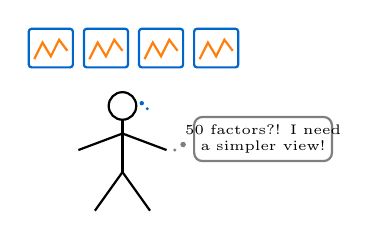
\begin{tikzpicture}[scale=0.7]
  % Trader stick figure
  \draw[thick] (1.5,3.5) circle (0.25);
  \draw[thick] (1.5,3.25) -- (1.5,2.3);
  \draw[thick] (1.5,3.0) -- (0.7,2.7);
  \draw[thick] (1.5,3.0) -- (2.3,2.7);
  \draw[thick] (1.5,2.3) -- (1.0,1.6);
  \draw[thick] (1.5,2.3) -- (2.0,1.6);
  % Multiple screens with charts
  \foreach \x in {-0.2, 0.8, 1.8, 2.8} {
    \draw[mlblue, thick, rounded corners=1pt] (\x,4.2) rectangle (\x+0.8,4.9);
    \draw[mlorange, thick] (\x+0.1,4.35) -- (\x+0.25,4.65) -- (\x+0.4,4.4) -- (\x+0.55,4.7) -- (\x+0.7,4.5);
  }
  % Sweat drops
  \fill[mlblue] (1.85,3.55) circle (0.04);
  \fill[mlblue] (1.95,3.45) circle (0.03);
  % Speech bubble
  \draw[mlgray, thick, rounded corners=3pt] (2.8,2.5) rectangle (5.3,3.3);
  \node[font=\tiny, text width=2.2cm, align=center] at (4.05,2.9) {50 factors?! I need a simpler view!};
  \fill[mlgray] (2.6,2.8) circle (0.05);
  \fill[mlgray] (2.45,2.7) circle (0.03);
\end{tikzpicture}
\end{columns}

\bottomnote{PCA was invented by Pearson (1901) and independently by Hotelling (1933) -- one of the oldest and most used tools in data science}
\end{frame}

%% SLIDE 3: Learning Objectives
\begin{frame}[t]{Learning Objectives}
\begin{columns}[T]
\column{0.95\textwidth}
\small
After this lecture, you will be able to:

\vspace{3mm}
\begin{enumerate}
\setlength{\itemsep}{6pt}
\item \highlight{Derive} PCA as variance maximization via eigendecomposition of the covariance matrix
\item \highlight{Analyze} scree plots and reconstruction error to select the number of components
\item \highlight{Evaluate} PCA's linear assumption using the Swiss roll and identify when non-linear methods are needed
\item \highlight{Apply} PCA to yield curve decomposition and portfolio risk reduction
\end{enumerate}

\vspace{3mm}
\begin{block}{Prerequisites}
\scriptsize Linear algebra (matrix multiplication, eigenvectors), basic statistics (variance, covariance), Python with scikit-learn.
\end{block}
\end{columns}

\bottomnote{All learning objectives target Bloom's level 4+ (analyze, evaluate, apply, derive)}
\end{frame}

%% SLIDE 4: What Is PCA in Plain English?
\begin{frame}[t]{What Is PCA in Plain English?}
\begin{columns}[T]
\column{0.55\textwidth}
\small
\textbf{The Camera Rotation Analogy}
\begin{compactlist}
\item Imagine a 3D cloud of data points viewed from a bad angle -- all points overlap
\item \highlight{PCA rotates the camera} to the angle that shows the widest spread
\item The first axis (PC1) captures the most variance
\item The second axis (PC2) is perpendicular and captures the next most
\end{compactlist}

\begin{block}{Key Insight}
\scriptsize PCA does not discard data -- it \emph{reorders} it by importance. You choose how many axes to keep.
\end{block}

\column{0.42\textwidth}
\vspace{2mm}
\footnotesize
\fcolorbox{mlpurple}{mllavender4}{\parbox{0.85\columnwidth}{%
\textbf{Key Terms}

\vspace{2mm}
\textbf{Principal Component}: a new axis (linear combination of original features)

\vspace{2mm}
\textbf{Explained Variance}: how much spread each PC captures

\vspace{2mm}
\textbf{Loadings}: weights showing each original feature's contribution to a PC

\vspace{2mm}
\textbf{Scree Plot}: bar chart of explained variance per PC
}}
\end{columns}

\bottomnote{PCA is a rotation followed by a projection -- the rotation is data-driven, choosing axes that maximize variance}
\end{frame}

%% SLIDE 5: Why Reduce Dimensions?
\begin{frame}[t]{Why Reduce Dimensions?}
\begin{columns}[T]
\column{0.95\textwidth}
\small
\textbf{Three Reasons to Compress Your Data}

\vspace{2mm}
\footnotesize
\begin{tabular}{@{}l p{10cm}@{}}
\toprule
\textbf{Reason} & \textbf{Details} \\
\midrule
\rowcolor{mllavender4}
\highlight{Visualization} & Project 50D data onto 2D to discover clusters, outliers, and trends that are invisible in tables \\
\highlight{Noise Reduction} & Low-variance directions are mostly noise. Discarding them improves signal-to-noise ratio. \\
\rowcolor{mllavender4}
\highlight{Speed} & Fewer features = faster training, lower memory, less overfitting. PCA from 1000 to 50 features can cut training time 20$\times$. \\
\bottomrule
\end{tabular}

\vspace{3mm}
\begin{block}{When NOT to Reduce}
\scriptsize If every feature is informative and uncorrelated, PCA will not help. PCA compresses correlated features -- if there is no redundancy, there is nothing to compress.
\end{block}
\end{columns}

\bottomnote{The curse of dimensionality: in high-D, all points become equidistant and nearest-neighbor methods fail}
\end{frame}

%% ================================================================
%% CORE ZONE -- METHOD (Slides 6-14)
%% ================================================================

%% SLIDE 6: Full Chart -- Original Clusters
\begin{frame}[t]{What Does the Data Look Like Before Reduction?}
\begin{center}

\includegraphics[width=0.65\textwidth]{06a_original_clusters/chart.pdf}
\end{center}

\bottomnote{High-dimensional data contains clusters that may be linearly separable -- PCA can reveal them by projecting onto the top PCs}
\end{frame}

%% SLIDE 7: Chart+Text -- Principal Components
\begin{frame}[t]{How Does PCA Find the Best Axes?}
\begin{columns}[T]
\column{0.55\textwidth}

\includegraphics[width=\textwidth]{02_principal_components/chart.pdf}

\column{0.42\textwidth}
\small
\textbf{Geometric Intuition}
\begin{compactlist}
\item \highlight{PC1}: direction of maximum variance in the data cloud
\item \highlight{PC2}: perpendicular to PC1, captures the next most variance
\item Each subsequent PC is orthogonal to all previous ones
\item The arrows show \emph{loadings} -- how each original feature contributes
\end{compactlist}

\begin{block}{Key Property}
\scriptsize PCs are uncorrelated by construction. This is why PCA is so useful -- it converts correlated features into independent components.
\end{block}
\end{columns}

\bottomnote{PCA finds the eigenvectors of the covariance matrix -- each eigenvector defines a principal component direction}
\end{frame}

%% SLIDE 8: Definition Block -- Variance Maximization
\begin{frame}[t]{The Variance Maximization Objective}
\begin{columns}[T]
\column{0.95\textwidth}
\small

\vspace{2mm}
\begin{block}{PCA Optimization Problem}
\[
\max_{\mathbf{w}} \; \mathbf{w}^T \mathbf{S} \mathbf{w} \quad \text{subject to} \quad \|\mathbf{w}\| = 1
\]
where $\mathbf{S} = \frac{1}{n-1}\mathbf{X}_c^T \mathbf{X}_c$ is the sample covariance matrix of centered data $\mathbf{X}_c$.
\end{block}

\vspace{2mm}
\textbf{Solution via Lagrange Multipliers}
\begin{compactlist}
\item Set up Lagrangian: $\mathcal{L} = \mathbf{w}^T \mathbf{S} \mathbf{w} - \lambda(\mathbf{w}^T\mathbf{w} - 1)$
\item Take derivative, set to zero: $\mathbf{S}\mathbf{w} = \lambda \mathbf{w}$
\item This is an eigenvalue equation -- $\mathbf{w}$ is an eigenvector of $\mathbf{S}$, $\lambda$ is the eigenvalue
\item The eigenvector with the largest eigenvalue = PC1 (direction of maximum variance)
\end{compactlist}
\end{columns}

\bottomnote{The eigenvalue $\lambda_k$ equals the variance explained by PC$k$ -- larger eigenvalue means more important component}
\end{frame}

%% SLIDE 9: Worked Example
\begin{frame}[t]{Worked Example: 2D to 1D by Hand}
\begin{columns}[T]
\column{0.95\textwidth}
\footnotesize
\textbf{Data}: 5 points in 2D: $(1,2)$, $(3,4)$, $(5,6)$, $(2,3)$, $(4,5)$

\vspace{2mm}
\textbf{Step 1: Center} -- Mean = $(3, 4)$. Centered: $(-2,-2)$, $(0,0)$, $(2,2)$, $(-1,-1)$, $(1,1)$

\vspace{1mm}
\textbf{Step 2: Covariance matrix}
\[
\mathbf{S} = \frac{1}{4}\begin{pmatrix} 10 & 10 \\ 10 & 10 \end{pmatrix} = \begin{pmatrix} 2.5 & 2.5 \\ 2.5 & 2.5 \end{pmatrix}
\]

\textbf{Step 3: Eigenvalues} -- $\det(\mathbf{S} - \lambda \mathbf{I}) = 0 \;\Rightarrow\; \lambda_1 = 5, \; \lambda_2 = 0$

\vspace{1mm}
\textbf{Step 4: Eigenvectors} -- $\mathbf{w}_1 = \frac{1}{\sqrt{2}}(1, 1)^T$ (PC1), $\mathbf{w}_2 = \frac{1}{\sqrt{2}}(1, -1)^T$ (PC2)

\vspace{1mm}
\textbf{Step 5: Project} -- $z_i = \mathbf{w}_1^T \mathbf{x}_i^c$: scores $= (-2\sqrt{2}, \; 0, \; 2\sqrt{2}, \; -\sqrt{2}, \; \sqrt{2})$

\vspace{1mm}
\textbf{Result}: PC1 explains 100\% of variance ($\lambda_1/(\lambda_1+\lambda_2) = 5/5 = 1.0$). All data lies on the line $y = x$.
\end{columns}

\bottomnote{This example is degenerate (all points on a line) -- real data has $\lambda_2 > 0$ but small, meaning PC2 captures residual noise}
\end{frame}

%% SLIDE 10: Chart+Text -- Scree Plot
\begin{frame}[t]{How Much Variance Does Each Component Explain?}
\begin{columns}[T]
\column{0.55\textwidth}

\includegraphics[width=\textwidth]{01_scree_plot/chart.pdf}

\column{0.42\textwidth}
\small
\textbf{Reading the Scree Plot}
\begin{compactlist}
\item Each bar shows the explained variance ratio of one PC
\item The cumulative line shows total variance retained
\item \highlight{90\% threshold}: keep enough PCs to cross this line
\item The ``elbow'' is where additional PCs add diminishing returns
\end{compactlist}

\begin{block}{Example}
\scriptsize If 3 PCs explain 92\% of variance in 50 features, you have compressed 50D to 3D with only 8\% information loss.
\end{block}
\end{columns}

\bottomnote{The scree plot is named after geological scree (rubble at the base of a cliff) -- stop where the cliff flattens}
\end{frame}

%% SLIDE 11: Chart+Text -- Reconstruction
\begin{frame}[t]{Reconstruction: Going Back to Original Space}
\begin{columns}[T]
\column{0.55\textwidth}

\includegraphics[width=\textwidth]{03_reconstruction/chart.pdf}

\column{0.42\textwidth}
\small
\textbf{The Reconstruction Formula}

\vspace{2mm}
Project to $k$ PCs and reconstruct:
\[
\hat{\mathbf{X}} = \mathbf{Z}\mathbf{W}_k^T + \boldsymbol{\mu}
\]

\begin{compactlist}
\item $\mathbf{Z}$: scores in PC space ($n \times k$)
\item $\mathbf{W}_k$: top $k$ eigenvectors ($p \times k$)
\item $\boldsymbol{\mu}$: original mean vector
\item \highlight{Reconstruction error} = variance of discarded PCs
\end{compactlist}

\begin{block}{Insight}
\scriptsize More components $\Rightarrow$ better reconstruction but less compression. The scree plot guides the tradeoff.
\end{block}
\end{columns}

\bottomnote{Reconstruction error equals $\sum_{j=k+1}^{p} \lambda_j$ -- the sum of eigenvalues of the discarded components}
\end{frame}

%% SLIDE 12: SVD and PCA
\begin{frame}[t]{SVD and PCA: Two Paths, One Answer}
\begin{columns}[T]
\column{0.95\textwidth}
\small
\textbf{Singular Value Decomposition}

\vspace{2mm}
Any centered data matrix can be decomposed as:
\[
\mathbf{X}_c = \mathbf{U}\boldsymbol{\Sigma}\mathbf{V}^T
\]

\begin{compactlist}
\item $\mathbf{V}$ (right singular vectors) = eigenvectors of $\mathbf{X}_c^T\mathbf{X}_c$ = PCA loadings
\item $\boldsymbol{\Sigma}$ (singular values) relate to eigenvalues: $\lambda_j = \sigma_j^2 / (n-1)$
\item $\mathbf{U}\boldsymbol{\Sigma}$ = PCA scores (projections onto principal components)
\end{compactlist}

\vspace{2mm}
\begin{block}{Why sklearn Uses SVD}
\scriptsize SVD is numerically more stable than computing $\mathbf{S} = \mathbf{X}^T\mathbf{X}/(n-1)$ explicitly. It avoids squaring condition numbers and works for $p > n$ (more features than samples).
\end{block}
\end{columns}

\bottomnote{In practice, always use sklearn's PCA which calls randomized SVD -- never compute the covariance matrix by hand for large datasets}
\end{frame}

%% SLIDE 13: Chart+Text -- Swiss Roll Failure
\begin{frame}[t]{When Does PCA Fail?}
\begin{columns}[T]
\column{0.55\textwidth}

\includegraphics[width=\textwidth]{05a_pca_swiss_roll/chart.pdf}

\column{0.42\textwidth}
\small
\textbf{The Linear Assumption}
\begin{compactlist}
\item PCA finds the best \emph{linear} projection
\item If structure is non-linear (curved manifold), PCA mixes up points
\item The Swiss roll: nearby points on the surface become far apart after PCA projection
\item Colors interleave instead of staying separated
\end{compactlist}

\begin{block}{Bridge to t-SNE}
\scriptsize When data lies on a curved surface, you need non-linear methods: t-SNE, UMAP, or kernel PCA.
\end{block}
\end{columns}

\bottomnote{PCA projects onto a hyperplane -- if the data manifold is curved, the projection flattens and destroys neighborhood structure}
\end{frame}

%% SLIDE 14: Full Chart -- PCA Cluster Projection
\begin{frame}[t]{PCA Projection Preserves Linear Clusters}
\begin{center}

\includegraphics[width=0.65\textwidth]{06b_pca_cluster_projection/chart.pdf}
\end{center}

\bottomnote{When clusters are linearly separable, PCA projection works well -- the top 2 PCs separate the groups cleanly}
\end{frame}

%% ================================================================
%% CORE ZONE -- SOLUTION (Slides 15-19)
%% ================================================================

%% SLIDE 15: Yield Curve PCA
\begin{frame}[t]{Yield Curve PCA: The Canonical Finance Example}
\begin{columns}[T]
\column{0.55\textwidth}
\small
\textbf{The Three Factors of Interest Rates}
\begin{compactlist}
\item Apply PCA to daily yield curve data (1Y, 2Y, 5Y, 10Y, 30Y maturities)
\item \highlight{PC1 ($\sim$85\%)}: Level -- all rates move together (parallel shift)
\item \highlight{PC2 ($\sim$10\%)}: Slope -- short rates move opposite to long rates
\item \highlight{PC3 ($\sim$3\%)}: Curvature -- the belly of the curve bows
\end{compactlist}

\begin{block}{Impact}
\scriptsize 3 components explain 98\% of yield curve variation. Fixed income risk management is built on this decomposition.
\end{block}

\column{0.42\textwidth}
\vspace{2mm}
\footnotesize
\fcolorbox{mlpurple}{mllavender4}{\parbox{0.85\columnwidth}{%
\textbf{Portfolio Hedging with PCA:}

\vspace{2mm}
Instead of tracking 10 maturities, hedge 3 factor exposures:

\vspace{2mm}
$\Delta P \approx D_1 \cdot \Delta\text{PC1}$

$\quad + D_2 \cdot \Delta\text{PC2}$

$\quad + D_3 \cdot \Delta\text{PC3}$

\vspace{2mm}
where $D_k$ = factor duration
}}
\end{columns}

\bottomnote{Litterman \& Scheinkman (1991) showed 3 PCA factors explain $>$98\% of US Treasury yield curve movements}
\end{frame}

%% SLIDE 16: Portfolio Risk Decomposition
\begin{frame}[t]{Portfolio Risk Decomposition}
\begin{columns}[T]
\column{0.95\textwidth}
\small
\textbf{From 50 Stocks to 5 Principal Portfolios}

\vspace{2mm}
\begin{enumerate}
\setlength{\itemsep}{4pt}
\item Compute daily returns matrix: $\mathbf{R}$ ($T \times 50$, where $T$ = trading days)
\item Standardize each column (zero mean, unit variance)
\item Run PCA: obtain eigenvectors $\mathbf{w}_1, \ldots, \mathbf{w}_{50}$
\item \highlight{PC1} = market factor (all stocks load positively) -- explains $\sim$40\% of variance
\end{enumerate}

\vspace{2mm}
\begin{block}{Interpretation}
\scriptsize Each PC defines a ``principal portfolio'' -- a linear combination of stocks. PC1 is the market, PC2 is often sector rotation (tech vs.\ energy), PC3 may capture momentum vs.\ value.
\end{block}
\end{columns}

\bottomnote{PCA on returns is the basis for statistical factor models -- an alternative to Fama-French style predefined factors}
\end{frame}

%% SLIDE 17: Choosing Number of Components
\begin{frame}[t]{Choosing the Number of Components}
\begin{columns}[T]
\column{0.47\textwidth}
\small
\textbf{Four Methods}
\begin{compactlist}
\item \highlight{Scree plot elbow}: visual inspection for the ``cliff edge''
\item \highlight{Kaiser criterion}: keep PCs with eigenvalue $> 1$ (when using correlation matrix)
\item \highlight{Cumulative variance}: keep enough PCs for 90--95\% of total variance
\item \highlight{Cross-validation}: choose $k$ that optimizes a downstream task (classification, regression)
\end{compactlist}

\column{0.50\textwidth}
\vspace{2mm}
\footnotesize
\begin{tabular}{@{}l l l@{}}
\toprule
\textbf{Method} & \textbf{Pro} & \textbf{Con} \\
\midrule
\rowcolor{mllavender4}
Scree elbow & Simple & Subjective \\
Kaiser & Automatic & Arbitrary \\
\rowcolor{mllavender4}
Cum.\ var.\ & Interpretable & Ignores task \\
CV & Task-optimal & Expensive \\
\bottomrule
\end{tabular}

\vspace{3mm}
\begin{block}{Practical Advice}
\scriptsize Start with the 90\% cumulative variance rule. If you have a downstream model, use cross-validation to fine-tune.
\end{block}
\end{columns}

\bottomnote{In sklearn: \texttt{PCA(n\_components=0.95)} automatically selects enough PCs to explain 95\% of variance}
\end{frame}

%% SLIDE 18: PCA as Preprocessing (fragile)
\begin{frame}[fragile,t]{PCA as Preprocessing for ML}
\begin{columns}[T]
\column{0.95\textwidth}
\small
\textbf{sklearn Pipeline: Scale $\rightarrow$ PCA $\rightarrow$ Classify}

\vspace{2mm}
\begin{verbatim}
from sklearn.pipeline import Pipeline
from sklearn.preprocessing import StandardScaler
from sklearn.decomposition import PCA
from sklearn.linear_model import LogisticRegression

pipe = Pipeline([
    ('scaler', StandardScaler()),
    ('pca',    PCA(n_components=0.95)),
    ('clf',    LogisticRegression())
])

pipe.fit(X_train, y_train)
print(f"Accuracy: {pipe.score(X_test, y_test):.3f}")
print(f"Components kept: {pipe['pca'].n_components_}")
\end{verbatim}

\vspace{1mm}
\begin{block}{Why This Works}
\scriptsize PCA removes noise (low-variance directions) and reduces multicollinearity. The classifier sees cleaner, lower-dimensional input.
\end{block}
\end{columns}

\bottomnote{Always scale before PCA -- features with larger units dominate the covariance matrix and distort the principal components}
\end{frame}

%% SLIDE 19: Interpreting Principal Components
\begin{frame}[t]{Interpreting Principal Components}
\begin{columns}[T]
\column{0.47\textwidth}
\small
\textbf{The Loadings Matrix}
\begin{compactlist}
\item Each PC is a weighted sum of original features
\item The weight of feature $j$ on PC $k$ is called the \highlight{loading} $w_{jk}$
\item Large positive loading: feature moves with the PC
\item Large negative loading: feature moves against the PC
\end{compactlist}

\column{0.50\textwidth}
\vspace{2mm}
\footnotesize
\textbf{Example: Stock Returns}

\vspace{2mm}
\begin{tabular}{@{}l r r@{}}
\toprule
\textbf{Stock} & \textbf{PC1} & \textbf{PC2} \\
\midrule
\rowcolor{mllavender4}
Apple & +0.18 & +0.35 \\
JPMorgan & +0.20 & $-0.28$ \\
\rowcolor{mllavender4}
Exxon & +0.15 & $-0.31$ \\
Google & +0.19 & +0.33 \\
\bottomrule
\end{tabular}

\vspace{2mm}
\scriptsize PC1: all positive $\Rightarrow$ \textbf{market factor}

PC2: tech positive, banks/energy negative $\Rightarrow$ \textbf{sector rotation}
\end{columns}

\bottomnote{Loadings are the eigenvector components -- they tell you what each PC ``means'' in terms of original features}
\end{frame}

%% ================================================================
%% CLOSING ZONE (Slides 20-25)
%% ================================================================

%% SLIDE 20: When to Use PCA
\begin{frame}[t]{When to Use PCA --- and When Not To}
\begin{columns}[T]
\column{0.47\textwidth}
\small
\textbf{\textcolor{mlgreen}{Pros}}
\begin{compactlist}
\item Interpretable components (loadings tell you what each PC means)
\item Fast: $O(np^2)$ or less with randomized SVD
\item Preserves global variance structure
\item Invertible: can reconstruct original data
\end{compactlist}

\column{0.50\textwidth}
\small
\textbf{\textcolor{mlred}{Cons}}
\begin{compactlist}
\item Linear only -- fails on curved manifolds (Swiss roll)
\item Sensitive to feature scaling (must standardize first)
\item Loses local neighborhood structure
\item Maximizes variance, which may not equal ``importance''
\end{compactlist}
\end{columns}

\vspace{3mm}
\begin{block}{Rule of Thumb}
\scriptsize Use PCA when you need preprocessing, interpretability, or compression. Switch to t-SNE/UMAP when you need to \emph{visualize} non-linear structure.
\end{block}

\bottomnote{PCA is the default first step in dimensionality reduction -- try it before anything more complex}
\end{frame}

%% SLIDE 21: Comparison Table
\begin{frame}[t]{PCA vs Factor Analysis vs Autoencoders}
\begin{columns}[T]
\column{0.95\textwidth}
\small

\vspace{1mm}
\footnotesize
\begin{tabular}{@{}l c c c@{}}
\toprule
\textbf{Property} & \textbf{PCA} & \textbf{Factor Analysis} & \textbf{Autoencoder} \\
\midrule
\rowcolor{mllavender4}
Linearity & Linear & Linear & Non-linear \\
Interpretability & High (loadings) & High (factors) & Low (black box) \\
\rowcolor{mllavender4}
Component selection & Scree/CV & Likelihood ratio & Architecture choice \\
Computational cost & Low & Medium & High (GPU) \\
\rowcolor{mllavender4}
Non-linear capability & No & No & Yes \\
Noise model & None & Explicit & Implicit \\
\rowcolor{mllavender4}
Reconstruction & Exact (with all PCs) & Approximate & Approximate \\
\bottomrule
\end{tabular}

\vspace{3mm}
\begin{block}{Practical Choice}
\scriptsize Start with PCA (fast, interpretable). If you need a latent variable model with noise, use Factor Analysis. If you need non-linear compression, use an autoencoder.
\end{block}
\end{columns}

\bottomnote{Factor Analysis assumes data = factors + noise; PCA makes no noise assumption -- it just maximizes explained variance}
\end{frame}

%% SLIDE 22: Hands-on Code (fragile)
\begin{frame}[fragile,t]{Hands-on: Decompose Portfolio Risk}
\begin{columns}[T]
\column{0.95\textwidth}
\small

\vspace{2mm}
\begin{verbatim}
from sklearn.decomposition import PCA
from sklearn.preprocessing import StandardScaler
import numpy as np

# Simulate 250 days x 50 stocks
np.random.seed(42)
returns = np.random.randn(250, 50) @ np.random.randn(50, 50) * 0.01

# Scale and fit PCA
scaler = StandardScaler()
X = scaler.fit_transform(returns)
pca = PCA().fit(X)

# Scree: cumulative explained variance
cumvar = np.cumsum(pca.explained_variance_ratio_)
k_90 = np.searchsorted(cumvar, 0.90) + 1
print(f"Components for 90% variance: {k_90}")
\end{verbatim}

\vspace{1mm}
\scriptsize Full notebook: \texttt{notebooks/L05\_pca.ipynb}
\end{columns}

\bottomnote{Try this yourself: load real stock returns from Yahoo Finance and see how many PCs you need for 90\% explained variance}
\end{frame}

%% SLIDE 23: Key Takeaways
\begin{frame}[t]{Key Takeaways}
\begin{columns}[T]
\column{0.47\textwidth}
\small
\textbf{Concepts}
\begin{compactlist}
\item PCA = eigenvectors of the covariance matrix
\item Eigenvalue = variance explained by that PC
\item Reconstruction error = discarded eigenvalue sum
\item Scree plot guides component selection
\end{compactlist}

\column{0.50\textwidth}
\small
\textbf{Practice}
\begin{compactlist}
\item Always standardize features before PCA
\item Use the scree plot 90\% rule as a starting point
\item Interpret loadings to understand what each PC means
\item Test with the Swiss roll: if PCA fails, try t-SNE or UMAP
\end{compactlist}
\end{columns}

\vspace{4mm}
\begin{block}{One-Sentence Summary}
\scriptsize PCA rotates your data to find the axes of maximum variance, letting you compress, denoise, and visualize high-dimensional data.
\end{block}

\bottomnote{PCA is a tool you will use in nearly every data science project -- master it.}
\end{frame}

%% SLIDE 24: Bridge to t-SNE
\begin{frame}[t]{What's Next: t-SNE for Visualization}
\begin{columns}[T]
\column{0.95\textwidth}
\small
\textbf{PCA Finds Global Axes. t-SNE Finds Local Neighborhoods.}

\vspace{3mm}
\begin{compactlist}
\item PCA captures the \highlight{directions of maximum spread} -- great for compression and preprocessing
\item But when the data lives on a curved manifold, PCA's linear projection fails
\item \highlight{t-SNE} minimizes the mismatch between high-D and low-D \emph{neighborhoods}
\item Result: clusters that PCA merges become clearly separated in t-SNE
\end{compactlist}

\vspace{3mm}
\begin{block}{Coming Up}
\scriptsize Next lecture: t-SNE's KL divergence objective, the perplexity parameter, the crowding problem, and UMAP as a modern alternative.
\end{block}
\end{columns}

\bottomnote{Best practice: run PCA first to reduce to 30--50 dimensions, then apply t-SNE on the PCA output for faster and more stable visualization}
\end{frame}

%% SLIDE 25: Closing XKCD
\begin{frame}[t]{Closing Thought}
\begin{center}
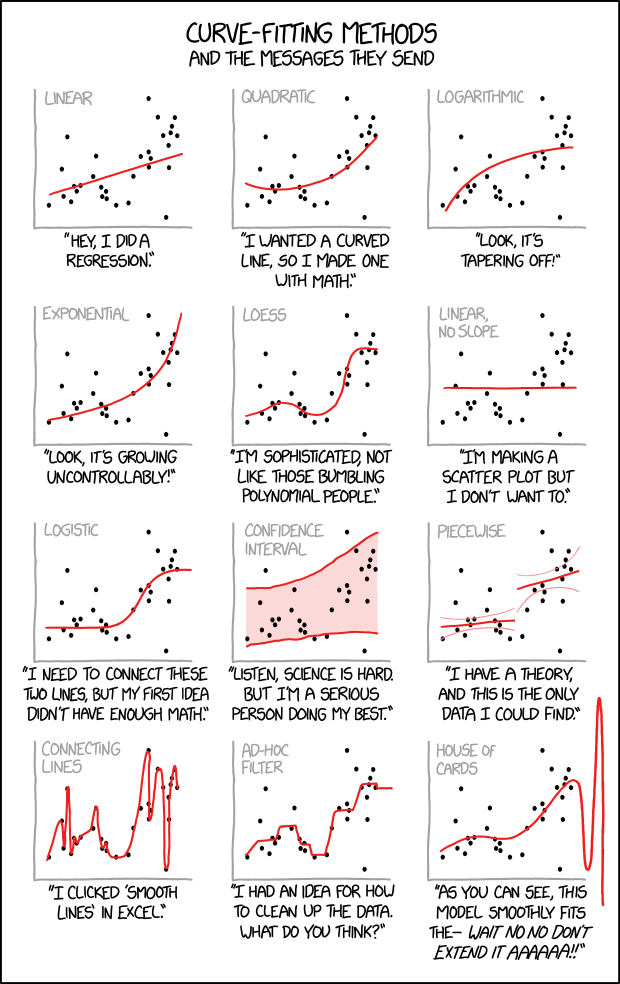
\includegraphics[width=0.6\textwidth,height=0.7\textheight,keepaspectratio]{images/2048_curve_fitting.png}
\end{center}

\bottomnote{XKCD \#2048 by Randall Munroe (CC BY-NC 2.5)}
\end{frame}

\end{document}
